\documentclass{beamer}

\usepackage[utf8]{inputenc}
%\usepackage{hyperref}
\usepackage[sort,compress]{cite}
\usepackage{algorithmic}
\usepackage[ruled,linesnumbered,lined]{algorithm2e}
\usepackage{booktabs}

\usepackage{amsfonts}%Usando fontes para conjuntos numéricos

%\usepackage{titlesec}
\usepackage{color,colortbl,multirow}
\usepackage{xy}
\usepackage{graphicx,url, amsmath, color}
\usepackage{graphicx}

\title{Projeto Segunda VA Visão Computacional\\
	Réplica do trabalho:\textbf{Simple face-detection algorithm based on minimum facial features}}
\author{\textbf{Aluno}: Ismael Cesar\\
		\textbf{Professor}: João Paulo}
\date{}
\begin{document}
\frame{
\begin{center}
	\maketitle
 
\end{center}
}

\frame{
	\frametitle{Introdução}
	\begin{itemize}
		\item Detecção de faces pode ser útil em várias aplicações dos dias atuais
		\item Tarefa de detectar pode ser muito custosa
		\item Procurar pelo mínimo de características faciais
		\begin{itemize}
			\item Pele
			\item Cabelo
		\end{itemize}
		\item Deixar detecção de face mais eficiente
	\end{itemize}
}

\frame{
	\frametitle{Conceitos Básicos}
	
	\begin{itemize}
		\item Uso de primitivas para computação de valores
		\item Modelo de cor RGB normalizado:	
		\begin{equation}
		\begin{split}
			r  = \frac{R}{R+G+B+\varepsilon} \\
			g  = \frac{G}{R+G+B+\varepsilon} \\
			b  = \frac{B}{R+G+B+\varepsilon}
		\end{split}
		\end{equation}	
	\end{itemize}			
}

\frame{
	\frametitle{Conceitos Básicos}
	
	\begin{itemize}
		\item Primitivas que definem o intervalos de cores para o canal $r$
		\begin{equation}
		\begin{split}
			F_1(r)  = -1.367r^2 + 1.0743r + 0.2 \\
			F_2(r)  = -0.776r^2 + 0.5601r + 0.18
		\end{split}
		\end{equation}
		\item Primitiva para computação dos tons de branco nos canais $r$ e $g$
		\begin{equation}
			White(r,g) = (r - 0.33)^2 + (g - 0.33)^2 
		\end{equation}
	\end{itemize}
}

\frame{
	\frametitle{Conceitos Básicos}
	\begin{itemize}
		\item Primitivas para relações entre o modelo de cor RGB e HSI
		$$
		\theta (R,G,B) = cos^{-1}\left( \frac{0.5((R-G)+(R-B))}{\sqrt{(R-G)^2 +(R-B)(G-R) }} \right)
		$$
		\\
		$$
	Hue(B,G,\theta) = 	\begin{cases}
						\theta,  \text{if } B \leq G \\
						360^\circ - \theta,  \text{if } B > G
						\end{cases}
		$$
		\\
		$$
		I(R,G,B) = 	\frac{1}{3} (R+G+B)
		$$
	\end{itemize}
}

\frame{
	\frametitle{Detecção de pele}
	
	\begin{itemize}
		\item Binarização da imagem segundo a equação:
		\resizebox{0.91\hsize}{!}{
		$
				SkinDetect = \begin{cases}
						1 , \text{ if }\left( g < F_1(r) \cap g > F_2(r) \cap White(r,g) > 0.001 \cap	
										(Hue(b,g,\theta) > \frac{4}{3}\pi \cup Hue(b,g,\theta) \leq \frac{\pi}{4} ) \right) \\
						0 , \text{ otherwise }
						\end{cases}
		$}
		
	\end{itemize}
}

\frame{
	\frametitle{Detecção de Cabelo}


	\begin{itemize}
	\item Binarização da imagem segundo a equação:
	\begin{equation}
	\resizebox{0.91\hsize}{!}{
	$
			HairDetect = \begin{cases}
					1 , \text{ if }\left( (I(r,g,b) < 0.313 \cap ((b-g)< 0.0588 \cup (b-r) < 0.0588))
									\cup (\frac{\pi}{4} < Hue(b,g,\theta) \leq \frac{\pi}{2} ) \right) \\
					0 , \text{ otherwise }
					\end{cases}	
	$
	}
	\end{equation}
		\end{itemize}
}

\frame{
	\frametitle{Quantização de pele e cabelo}
	
	\begin{itemize}
		\item Operações morfológicas
		\item Elemento estruturante de tamanhos:
		\begin{itemize}
			\item $ 10 \times 10 $ para detecção de face
			\item $ 3 \times  3$  para detecção de cabelo
			\item Empíricamente os resultados são melhores
		\end{itemize}
	\end{itemize}
}

\frame{
	\frametitle{Quantização de pele e cabelo}
	\begin{itemize}
		\item Computação dos componentes conexos e suas características
		\item Aplicação do filtro de tamanho
		\begin{itemize}
			\item Componente conexo com área menor que um limiar é descartado
		\end{itemize}
		\item Vértices dos retângulos que contém os componentes conexos são computados
	\end{itemize}
}

\frame{
	\frametitle{Detecção}
	\begin{itemize}
		\item União de todas as features
		\item É calculada a intersecção entre retângulos de componentes conexos
		\begin{itemize}
			\item[*] Intersecção de maior área tem mais prioridade
		\end{itemize}
		\item Caso não haja intesecção:
		\begin{itemize}
			\item Algoritmo considera que nenhuma face foi encontrada
		\end{itemize}		
	\end{itemize}
}

\frame{
	\frametitle{Resultados}
	\begin{figure}[htb]
\resizebox{.9 \textwidth}{!}{
\begin{tabular}{cccccc}

	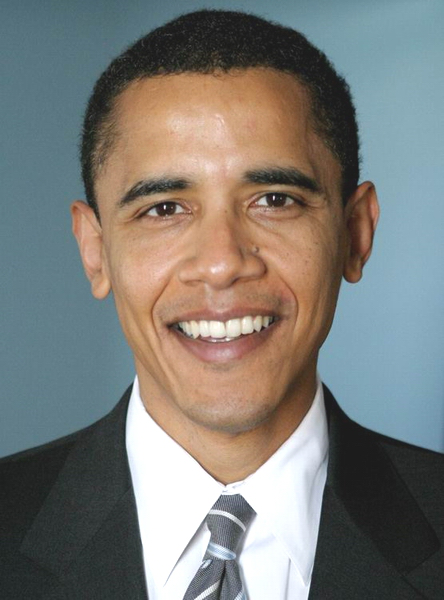
\includegraphics[scale=0.3]{images/Original.png}
  &

	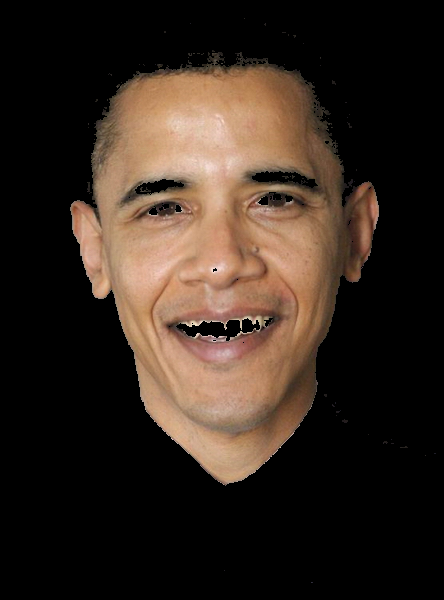
\includegraphics[scale=0.3]{images/skinDetect.png}

&

	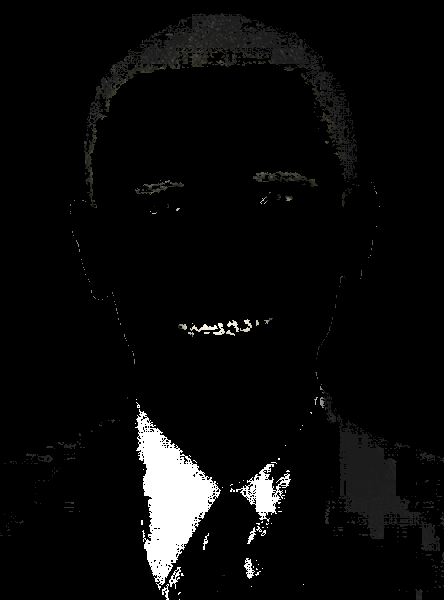
\includegraphics[scale=0.3]{images/hairDetect.png}

&

	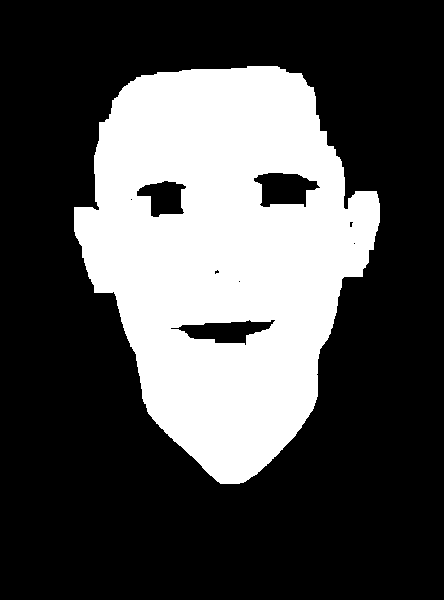
\includegraphics[scale=0.3]{images/skinQuantization.png}

&

	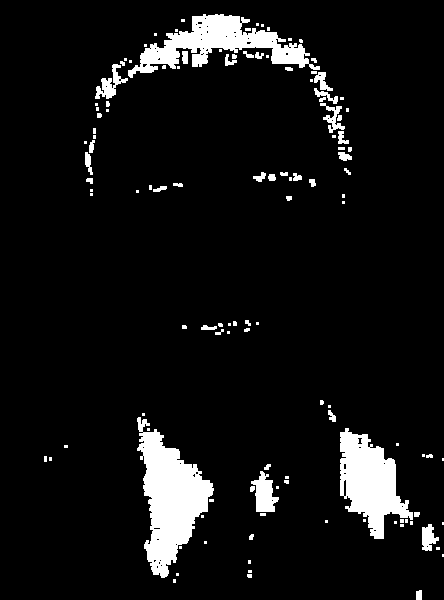
\includegraphics[scale=0.3]{images/hairQuantization.png}

&

	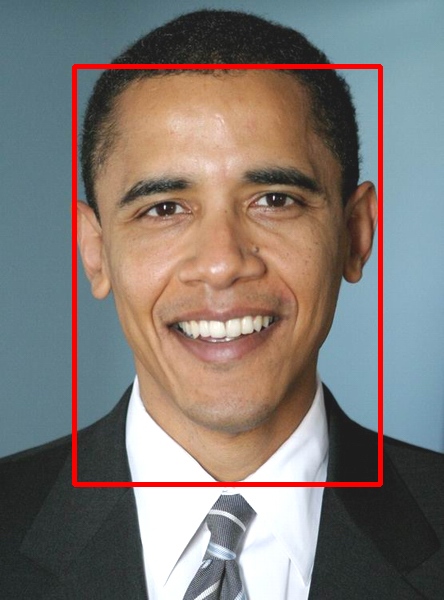
\includegraphics[scale=0.3]{images/Detection.png}
\\
Original & Skin Detection & Hair Detection & Skin Quantization & Hair Quantization & Detection\\
\end{tabular}
}	
\end{figure}
}

%Slide detecções espúrias
\frame{
	\frametitle{Resultados}
	\framesubtitle{Detecções espúrias}
	
	\begin{figure}[h]
\resizebox{.95 \textwidth}{!}{
\begin{tabular}{cccccc}

	
\includegraphics[scale=0.3]{images/OriginalSpurious.png}
  &

	
\includegraphics[scale=0.3]{images/skinDetectSpurious.png}

&

	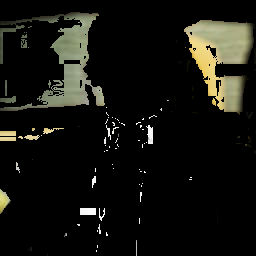
\includegraphics[scale=0.3]{images/hairDetectSpurious.png}

&

	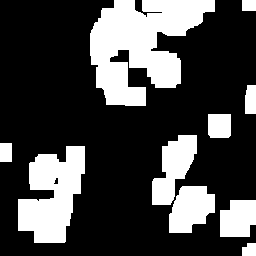
\includegraphics[scale=0.3]{images/skinQuantizationSpurious.png}

&

	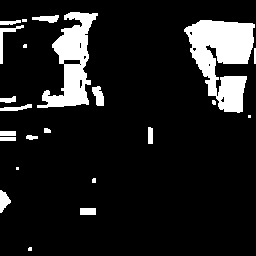
\includegraphics[scale=0.3]{images/hairQuantizationSpurious.png}

&

	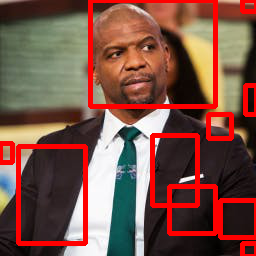
\includegraphics[scale=0.3]{images/DetectionSpurious.png}
\\
Original & Skin Detection & Hair Detection & Skin Quantization & Hair Quantization & Detection\\
\end{tabular}
}	
\end{figure} 
}%Slide detecções espúrias

\frame{
	\frametitle{Conclusões}
	\begin{itemize}
		\item Alta dependência das cores na imagem pode resultar em muitos outliers
		\item A presença de elementos com mesmo tom de pele ou de cabelo perto de faces de verdade podem interferir causando uma detecção pouco precisa
		\begin{figure}[htb]
\resizebox{1 \textwidth}{!}{
\begin{tabular}{cc}

	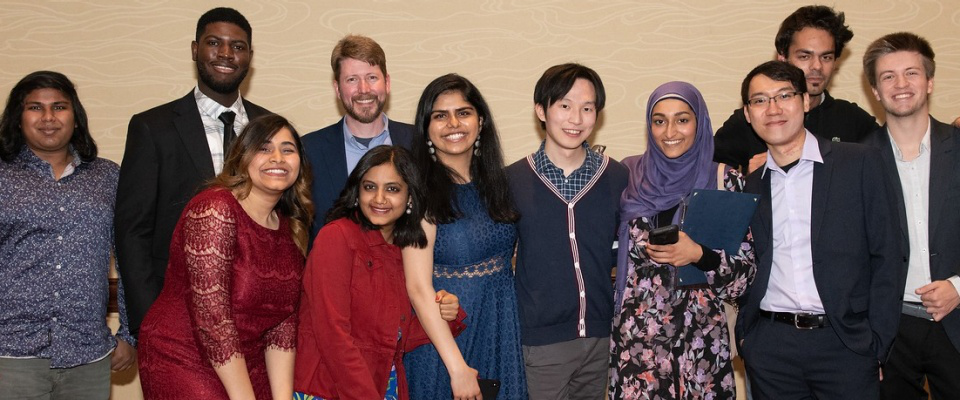
\includegraphics[scale=0.3]{images/OriginalSpurious2.png}
  &

	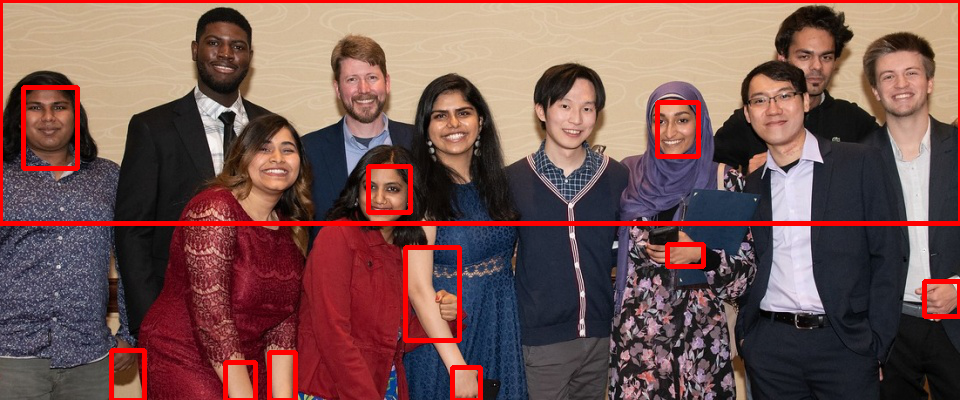
\includegraphics[scale=0.3]{images/DetectionSpurious2.png}
\\
Original &  Detection\\
\end{tabular}
}	
\end{figure} 
	\end{itemize}
}

\frame{
	\frametitle{Trabalhos futuros}
	\framesubtitle{Ainda há esperança}
	
	\begin{itemize}
		\item Utilizar esse algortimo como heuristica para algoritmos de aprendizagem de máquina que efetuam detecção de faces
		\begin{itemize}
			\item Definição de regiões de interesse
			\item Sem a necessidade de fazer uma varredura na imagem inteira
		\end{itemize}
	\end{itemize}
}

\frame{
	\begin{center}
	\resizebox{0.95 \textwidth}{!}{Obrigado!}
	\end{center}
}

\end{document}